% !TeX root = RJwrapper.tex
\title{Changes in R}
\author{by Tomas Kalibera, Sebastian Meyer, and Kurt Hornik}

\maketitle

\abstract{%
We present important changes in the development version of R (referred to as R-devel, to become R 4.3). Some statistics on bug tracking activities in 2022 are also provided.
}

\hypertarget{r-devel-selected-changes}{%
\section{R-devel selected changes}\label{r-devel-selected-changes}}

R 4.3.0 is due to be released around April 2023. The following gives a
selection of the most important changes in R-devel, which are likely to
appear in the new release.

\hypertarget{dates-and-times}{%
\subsection{Dates and times}\label{dates-and-times}}

There are a number of (robustness) improvements in the handling of dates
and times. These include warnings about extrapolation for datetimes before
1902/1900, finer control for padding when printing years, improved detection
of offset with \texttt{strftime()} (\texttt{\%z}), inclusion of system time zone and
information on timezone support implementation in \texttt{sessionInfo()}, more
robust handling of hand-crafted \texttt{POSIXlt} objects, optional support for
using system timezone support on recent macOS, improved detection of the
system time zone on Windows and improved default tick locations and default
formats in \texttt{axis.Date()} and \texttt{axis.POSIXct()}.

\hypertarget{encoding-support}{%
\subsection{Encoding support}\label{encoding-support}}

\begin{itemize}
\item
  Performance of regular expression operations in R has been improved by
  reducing the costs of encoding conversions. With \texttt{perl=FALSE}, all
  inputs have to be converted to UTF-16 or UTF-32, and the conversion is
  now faster. With \texttt{perl=TRUE}, performance has been improved by opting
  out from duplicate checks for UTF-8 validity in PCRE2. With
  \texttt{fixed=TRUE}, performance has been improved by taking advantage of the
  properties of UTF-8. One of the motivations for the speedups was to
  reduce the incentive for using \texttt{useBytes=TRUE} with regular expression
  operations, which often leads to incorrect results or errors due to
  producing invalid strings.

  See \href{https://blog.r-project.org/2022/07/12/speedups-in-operations-with-regular-expressions}{Speedups in operations with regular expressions}
  for more information.
\item
  The support for encoding-agnostic string operations in R using the
  ``bytes'' encoding has been improved. It is now possible to read a text
  file directly as bytes. Regexp operations, when creating new strings by
  splitting or substituting, now also flag them as ``bytes'' when any of the
  input has been flagged as such. This simplifies encoding-agnostic parsing
  of files such as \texttt{DESCRIPTION}. \texttt{iconv(,from="")} now respects the
  encoding flag of the input string, making it easier to recover from
  type-instability in return values of regular expression operations.
  Improving the support for encoding-agnostic operations using the ``bytes''
  encoding comes together with stricter checking of validity of real
  strings in a character encoding, e.g.~``unknown/native'', which has been
  helpful in revealing user errors. In the long term, it should also help
  to simplify encoding support in R.

  See \href{https://blog.r-project.org/2022/10/10/improvements-in-handling-bytes-encoding}{Improvements in handling bytes encoding}
  for more information. The blog includes a detailed introduction to string and
  encoding support in R.

  See \href{https://blog.r-project.org/2022/06/27/why-to-avoid-\%5Cx-in-regular-expressions/}{Why to avoid \textbackslash x in regular expressions}
  for related information on the danger of using \texttt{\textbackslash{}x} escapes in regular
  expressions, which leads to errors, that are now more likely to be
  detected by R. This is closely related as \texttt{\textbackslash{}x} is a common way to
  create invalid strings.
\end{itemize}

\hypertarget{graphics}{%
\subsection{Graphics}\label{graphics}}

\begin{itemize}
\item
  The grDevices and grid packages have new functions for rendering typeset
  glyphs, primarily: \texttt{grDevices::glyphInfo()} and \texttt{grid::grid.glyph()}.
\item
  The behaviour of compositing operators in \texttt{grid::grid.group()} has been
  tweaked to allow consistency across graphics devices.
\item
  The \texttt{grDevices::quartz()} device will support gradient fills, pattern
  fills, clipping paths, masks, compositing operators, affine
  transformations, stroked/filled paths, and glyphs. To be soon merged to
  R-devel.
\end{itemize}

\hypertarget{accessibility-on-windows}{%
\subsection{Accessibility on Windows}\label{accessibility-on-windows}}

\begin{itemize}
\item
  \texttt{Rgui} console on Windows now works better with the open-source NVDA
  screen reader when the ``full'' blinking cursor is selected. This is due to
  improved implementation of the console cursor (when it is displayed and
  hidden with respect to application startup and window focus) on which
  makes it easier for the screen reader to detect where the cursor is.
  Previously, NVDA was not able to read out the character under the cursor
  moved by the arrow keys.
\item
  The drop-field GraphApp control, which is used in the \texttt{Rgui} configuration
  editor, has been extended so that it can be left by pressing the TAB key,
  so without using the mouse.
\item
  GraphApp has been extended to allow reverse-order navigation through the
  controls using Shift+TAB key, which can now be done also in the \texttt{Rgui}
  configuration editor.
\end{itemize}

\hypertarget{other-selected-changes}{%
\subsection{Other selected changes}\label{other-selected-changes}}

\begin{itemize}
\item
  Using vectors of more than one element with the logical operators \texttt{\&\&}
  and \texttt{\textbar{}\textbar{}} will give an error in R 4.3.0 (a warning in R 4.2.x, a check
  error since R 3.6.0).
\item
  Support for working with concordances has been extended from
  Sweave to help files. A concordance is a mapping between lines in an
  intermediate file (e.g., \texttt{.tex} or \texttt{.html}) and lines in the
  corresponding input file (e.g., \texttt{.Rnw} or \texttt{.Rd}), which, for example, allows
  relating problems in the intermediate file to the source file from which
  it was generated.

  See \href{https://blog.r-project.org/2022/10/20/concordances}{Concordances} for more
  information.
\item
  The implementation of the sampling profiler, \texttt{Rprof()}, has been
  improved. On macOS, the profiler is now more robust against high load on
  the system by using low-level Mach API to avoid a race condition between
  initialization of pthread data and arrival of a profiler signal. This
  race condition could lead to a live-lock when the system has been
  overloaded due to a too short profiling interval. As an additional
  measure, \texttt{Rprof()} now refuses to use a too short profiling interval,
  which in the first place would lead to incorrect profiling results. To
  prevent a deadlock seen on Windows, the profiler has been rewritten to
  avoid using C runtime functions while the main thread is suspended.
\item
  Package installation now uses C++17 as the default C++ standard (and
  there is initial support for C++23). Also, there now is support for
  a package to indicate the version of the C standard which should be
  used to compile it, and for the installing user to specify this. In
  most cases, C17 (a ``bug-fix'' of C11) is used by default.
\item
  Producing PDF manuals (\texttt{R\ CMD\ Rd2pdf}) now loads standard AMS-LaTeX
  packages for greater coverage of math commands in Rd equations
  (e.g., \texttt{\textbackslash{}lVert} and \texttt{\textbackslash{}text}), and for consistency with the
  enhanced HTML math rendering introduced in R 4.2.0. This change has been
  backported to the R 4.2 release branch.
\item
  The \texttt{"repos"} option is now initialized from the \texttt{repositories} file,
  see \texttt{?R\_REPOSITORIES}, allowing the default CRAN mirror to be set therein.
\end{itemize}

\hypertarget{bug-statistics-for-2022}{%
\section{Bug statistics for 2022}\label{bug-statistics-for-2022}}

Summaries of bug-related activities over the past year were derived from the
database underlying \href{https://bugs.R-project.org/}{R's Bugzilla system}.
Overall, 180 new bugs or requests for enhancements were reported,
171 reports were closed, and 869 comments (on any report) were added
by a total of 123 contributors.
This amounts to one report/closure every other day,
and 2--3 comments per day.
The numbers of reports, closures and comments are about 20\% lower than in
2021,
whereas the number of contributors stayed the same.
High bug activity in 2021 had largely been driven by dedicated efforts of
several contributors in reviewing old reports.

\begin{figure}

{\centering 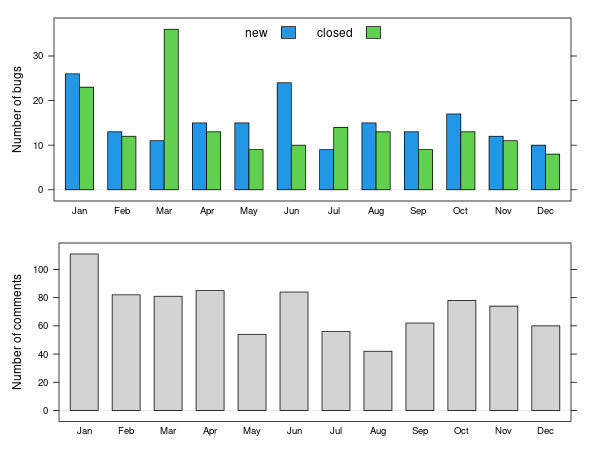
\includegraphics[width=1\linewidth]{bzstats_mon} 

}

\caption{Bug tracking activity by month in 2022}\label{fig:bzstatsmon}
\end{figure}

\begin{figure}

{\centering 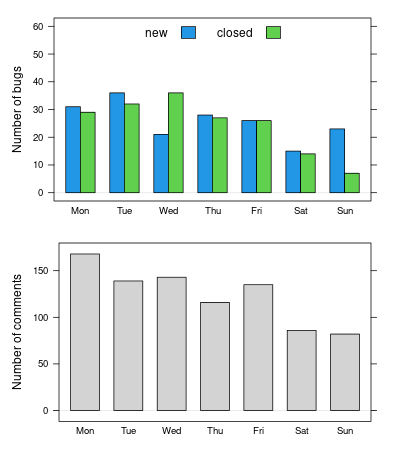
\includegraphics[width=0.6\linewidth]{bzstats_wd} 

}

\caption{Bug tracking activity by weekday in 2022}\label{fig:bzstatswd}
\end{figure}

Figures \ref{fig:bzstatsmon} and \ref{fig:bzstatswd} show statistics for the numbers of new reports,
closures and comments by calendar month and weekday, respectively, in 2022.
The frequency of new reports was relatively stable over the year with minor
peaks in January and June. There tended to be more new reports than
closures, except for July and especially March with a revived effort
to deal with old reports, including 9 related to the \CRANpkg{nlme} package,
which is also maintained by the R Core Team.

The top 5 components reporters have chosen for their reports were
``Misc'', ``Language'', ``Low-level'', ``Documentation'', and ``Wishlist'',
which is the same set as in 2021. Many reports are suggestions for
enhancements and placed either in the ``Wishlist'' or in a
specific component but with severity level set to ``enhancement''.
Bug discussions led to an average of 72 comments per month, with a minimum
of 42 in August and a maximum of 111 in January.
From the numbers in Figure \ref{fig:bzstatswd} we see that the R community is also active during
weekends, though at a lower frequency.

\hypertarget{acknowledgements}{%
\section*{Acknowledgements}\label{acknowledgements}}
\addcontentsline{toc}{section}{Acknowledgements}

Tomas Kalibera's work on the article and R development has received funding
from the National Science Foundation award 1925644.


\address{%
Tomas Kalibera\\
R Core\\%
Czechia\\
%
%
%
\href{mailto:Tomas.Kalibera@R-project.org}{\nolinkurl{Tomas.Kalibera@R-project.org}}%
}

\address{%
Sebastian Meyer\\
Friedrich-Alexander-Universität Erlangen-Nürnberg\\%
Germany\\
%
%
\textit{ORCiD: \href{https://orcid.org/0000-0002-1791-9449}{0000-0002-1791-9449}}\\%
\href{mailto:Sebastian.Meyer@R-project.org}{\nolinkurl{Sebastian.Meyer@R-project.org}}%
}

\address{%
Kurt Hornik\\
WU Wirtschaftsuniversität Wien\\%
Austria\\
%
%
\textit{ORCiD: \href{https://orcid.org/0000-0003-4198-9911}{0000-0003-4198-9911}}\\%
\href{mailto:Kurt.Hornik@R-project.org}{\nolinkurl{Kurt.Hornik@R-project.org}}%
}
